\documentclass[border=2pt,tikz]{standalone}
\usepackage[T1]{fontenc}
% Nature Portfolio / Scientific Data shared TikZ style for IRexp figures.
% Width: 183 mm double-column. Typography: Helvetica-class (phv).
\RequirePackage{tikz}
\RequirePackage{pgfplots}
\RequirePackage{xcolor}
\RequirePackage{helvet}
\IfFileExists{sansmathfonts.sty}{\RequirePackage{sansmathfonts}}{}
\renewcommand{\familydefault}{\sfdefault}
\pgfplotsset{compat=1.18}
\usetikzlibrary{
  arrows.meta,calc,positioning,fit,shapes.geometric,shapes.misc,
  backgrounds,shadows.blur,patterns,decorations.pathreplacing
}

% ---- Paul Tol / NMRexp-matched palette ----
\definecolor{nmrBlue}{HTML}{4A7EBB}
\definecolor{nmrBlueDark}{HTML}{2E5F8F}
\definecolor{nmrBlueLight}{HTML}{A8C8E8}
\definecolor{nmrPeach}{HTML}{E8B48C}
\definecolor{nmrNavy}{HTML}{1B3D5C}
\definecolor{nmrRed}{HTML}{C44E52}
\definecolor{nmrGreen}{HTML}{3D8B5E}
\definecolor{nmrOrange}{HTML}{D97B32}
\definecolor{ink}{HTML}{1A1A1A}
\definecolor{muted}{HTML}{7A7F85}
\definecolor{note}{HTML}{5C636A}
\definecolor{faint}{HTML}{E8EAEC}
\definecolor{ghost}{HTML}{C5C9CD}
\definecolor{tintBlue}{HTML}{EEF3F8}
\definecolor{tintGreen}{HTML}{EAF4EE}

\newcommand{\NatureFont}{\fontfamily{phv}\selectfont}
\newcommand{\PanelLabel}[1]{%
  {\NatureFont\bfseries\fontsize{8}{9.6}\selectfont #1}%
}
\newcommand{\FigBody}{\NatureFont\fontsize{7}{8.4}\selectfont}
\newcommand{\FigSmall}{\NatureFont\fontsize{5.5}{6.6}\selectfont}
\newcommand{\FigAxis}{\NatureFont\fontsize{7}{8.4}\selectfont}

\tikzset{
  nature arrow/.style={
    -{Latex[length=1.6mm,width=1.3mm]},
    line width=0.55pt, ink
  },
  nature arrow grey/.style={
    -{Latex[length=1.6mm,width=1.3mm]},
    line width=0.5pt, note
  },
  stage card/.style={
    draw=nmrBlueDark, line width=0.7pt, rounded corners=2.2pt,
    fill=white, inner sep=3pt, align=center, font=\FigBody
  },
  stage header/.style={
    fill=nmrBlueDark, text=white, font=\FigBody\bfseries,
    rounded corners=2.2pt, inner sep=2.5pt, align=center
  },
  soft card/.style={
    draw=ghost, line width=0.55pt, rounded corners=2.2pt,
    fill=white, inner sep=3.5pt, align=left, font=\FigBody
  },
}

\pgfplotsset{
  nature axis/.style={
    tick label style={font=\FigSmall, /pgf/number format/assume math mode},
    label style={font=\FigAxis\bfseries},
    title style={font=\FigBody\bfseries, color=ink},
    axis line style={ink, line width=0.5pt},
    tick style={ink, line width=0.45pt},
    major grid style={faint, line width=0.35pt},
    axis x line=bottom,
    axis y line=left,
    enlarge x limits=false,
    clip=false,
  },
  nature hbar/.style={
    nature axis,
    xbar,
    bar width=7pt,
    y=data,
    nodes near coords,
    every node near coord/.append style={
      font=\FigSmall, ink, anchor=west, /pgf/number format/fixed,
      /pgf/number format/1000 sep={,}
    },
    xtick=\empty,
    axis x line=none,
    y axis line style={ink, line width=0.55pt},
    ytick style={draw=none},
    y tick label style={font=\FigBody, ink, anchor=east},
    grid=major x,
    xmin=0,
  },
}

% Auto-generated from frozen_plot_data.json — do not edit by hand.
\newcommand{\IRexpTotal}{121233}
\newcommand{\IRexpStruct}{43060}
\newcommand{\IRexpCommercial}{88545}
\newcommand{\IRexpNMR}{87075}
\newcommand{\IRexpPMC}{119345}
\newcommand{\IRexpChemotion}{1888}
\newcommand{\IRexpNC}{21823}
\newcommand{\IRexpEmpty}{8963}
\newcommand{\IRexpSA}{1897}
\newcommand{\IRexpOther}{5}
\newcommand{\IRexpQuad}{33201}
\newcommand{\NMRexpN}{3370987}
\newcommand{\SDBSN}{54100}
\newcommand{\NISTN}{17000}
\newcommand{\BandMedian}{9}
\newcommand{\TxMAE}{0.0049}
\newcommand{\BandRecallPool}{0.9903}
\newcommand{\ListMatchPool}{0.9848}
\newcommand{\FailRate}{0.0321}

% Band histogram coordinates (x,y)
\newcommand{\BandHistCoords}{
(4,24556)
(6,22989)
(8,18726)
(10,14534)
(12,9959)
(14,7368)
(16,5241)
(18,3899)
(20,3017)
(22,2202)
(24,1822)
(26,1426)
(28,1069)
(30,826)
(32,698)
(34,534)
(36,386)
(38,408)
(40,298)
(42,250)
}

% Element bars
\newcommand{\ElementCommonCoords}{
(43047,8)% C
(38870,7)% O
(36292,6)% N
(12258,5)% S
(5939,4)% F
(7675,3)% Cl
(3923,2)% Br
(959,1)% Si
(859,0)% P
}
\newcommand{\ElementRareCoords}{
(904,8)% I
(270,7)% B
(384,6)% Se
(119,5)% Fe
(73,4)% Te
(64,3)% Sn
(1,2)% Ge
(16,1)% Na
(24,0)% K
}
\newcommand{\ElementCommonLabels}{C,O,N,S,F,Cl,Br,Si,P}
\newcommand{\ElementRareLabels}{I,B,Se,Fe,Te,Sn,Ge,Na,K}
\newcommand{\ElC}{43047}
\newcommand{\ElO}{38870}
\newcommand{\ElN}{36292}
\newcommand{\ElS}{12258}
\newcommand{\ElF}{5939}
\newcommand{\ElCl}{7675}
\newcommand{\ElBr}{3923}
\newcommand{\ElSi}{959}
\newcommand{\ElP}{859}
\newcommand{\ElI}{904}
\newcommand{\ElB}{270}
\newcommand{\ElSe}{384}
\newcommand{\ElFe}{119}
\newcommand{\ElTe}{73}
\newcommand{\ElSn}{64}
\newcommand{\ElGe}{1}
\newcommand{\ElNa}{16}
\newcommand{\ElK}{24}
\newcommand{\TxErrMedian}{0.0}
\newcommand{\TxErrCoords}{
(0.0250,196)
(0.0750,0)
(0.1250,0)
(0.1750,0)
(0.2250,0)
(0.2750,0)
(0.3250,0)
(0.3750,0)
(0.4250,1)
(0.4750,0)
(0.5250,1)
(0.5750,1)
(0.6250,0)
(0.6750,0)
(0.7250,0)
(0.7750,1)
(0.8250,0)
(0.8750,0)
(0.9250,0)
(0.9750,0)
(1.0250,0)
}
\newcommand{\TxErrBinWidth}{0.05000}
\newcommand{\PaperRecallMedian}{1.0}
\newcommand{\PaperRecallCoords}{
(0.0250,3)
(0.0750,0)
(0.1250,0)
(0.1750,0)
(0.2250,0)
(0.2750,0)
(0.3250,0)
(0.3750,0)
(0.4250,1)
(0.4750,0)
(0.5250,0)
(0.5750,0)
(0.6250,0)
(0.6750,0)
(0.7250,0)
(0.7750,0)
(0.8250,0)
(0.8750,1)
(0.9250,0)
(0.9750,0)
(1.0250,115)
}
\newcommand{\PaperRecallBinWidth}{0.05000}
\newcommand{\ListMatchMedian}{1.0}
\newcommand{\ListMatchCoords}{
(0.0250,4)
(0.0750,0)
(0.1250,0)
(0.1750,0)
(0.2250,0)
(0.2750,0)
(0.3250,0)
(0.3750,0)
(0.4250,0)
(0.4750,0)
(0.5250,1)
(0.5750,0)
(0.6250,2)
(0.6750,1)
(0.7250,1)
(0.7750,0)
(0.8250,1)
(0.8750,0)
(0.9250,0)
(0.9750,0)
(1.0250,109)
}
\newcommand{\ListMatchBinWidth}{0.05000}
\newcommand{\FailCtMedian}{0.0}
\newcommand{\FailCtCoords}{
(0.1250,271)
(0.3750,0)
(0.6250,0)
(0.8750,0)
(1.1250,9)
(1.3750,0)
(1.6250,0)
(1.8750,0)
(2.1250,0)
(2.3750,0)
}
\newcommand{\FailCtBinWidth}{0.25000}


\begin{document}
\NatureFont
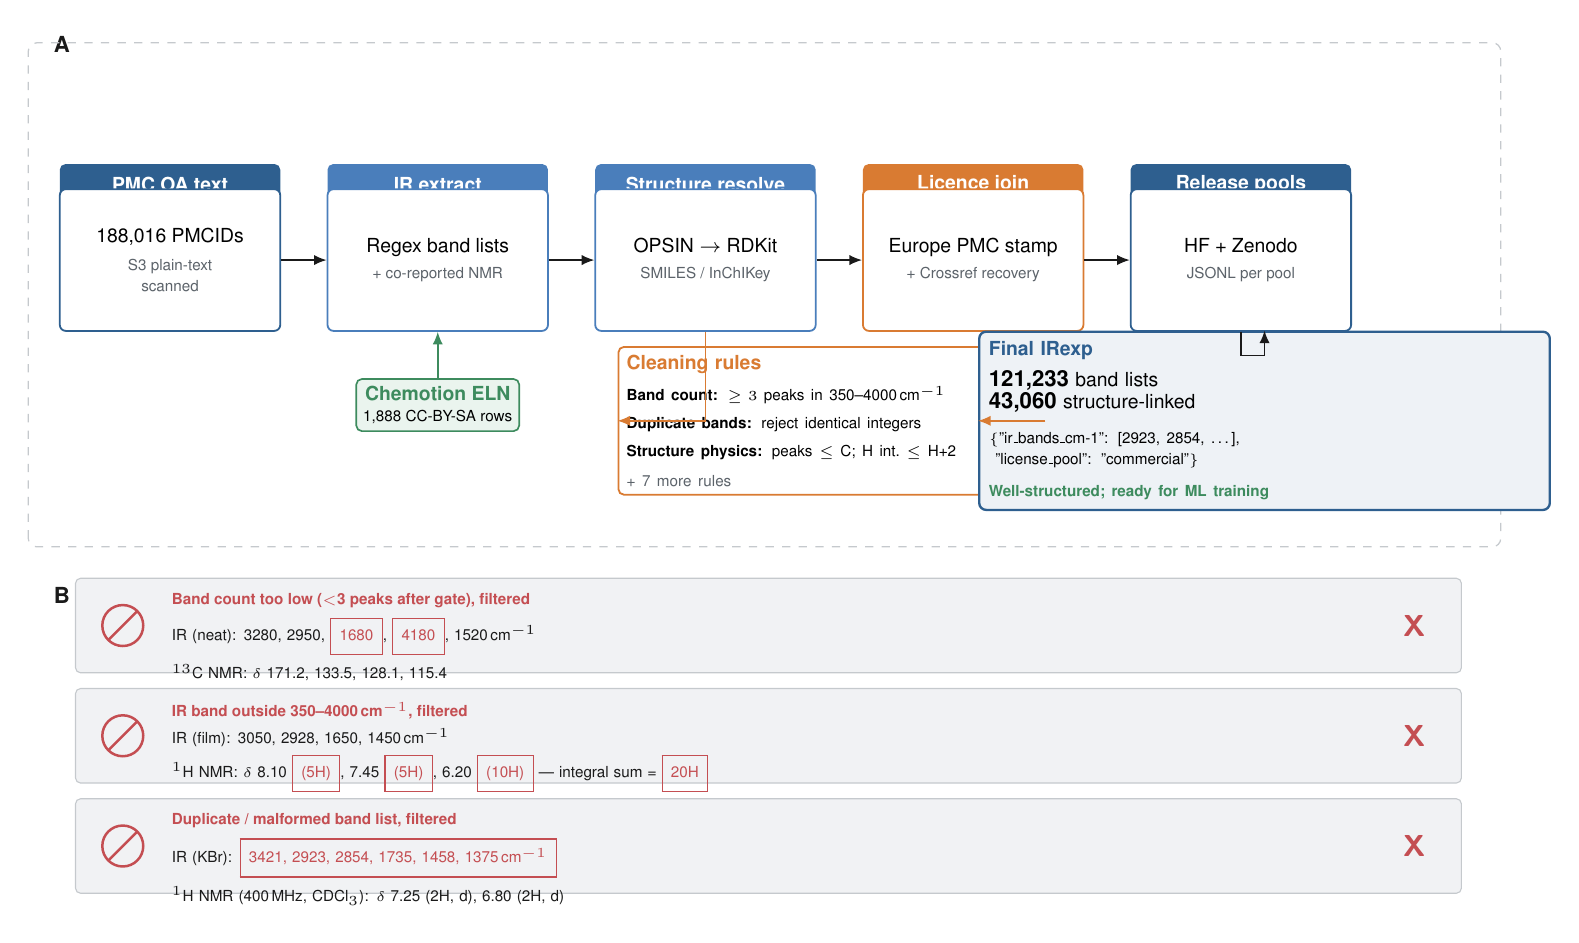
\begin{tikzpicture}[x=1mm,y=1mm,
  card/.style={
    draw=#1, line width=0.65pt, rounded corners=2.2pt, fill=white,
    minimum width=28mm, minimum height=18mm, align=center, font=\FigBody, inner sep=2pt
  },
  hdr/.style={
    fill=#1, text=white, font=\FigBody\bfseries, rounded corners=2pt,
    minimum width=28mm, minimum height=5.2mm, inner sep=1.5pt, align=center
  }]

  \node[font=\fontsize{9}{11}\selectfont\bfseries,ink,anchor=north west] at (0,118) {\PanelLabel{A}};

  % Outer dashed frame for panel A
  \draw[ghost,line width=0.45pt,dashed,rounded corners=3pt] (-2,52) rectangle (185,116);

  % Stage positions
  \def\Y{98}
  % PMC
  \node[hdr=nmrBlueDark] (h1) at (16,\Y) {PMC OA text};
  \node[card=nmrBlueDark, below=0pt of h1, yshift=2.2mm] (c1) {%
    188{,}016 PMCIDs\\[0.6mm]
    {\FigSmall\color{note}S3 plain-text}\\[-0.2mm]
    {\FigSmall\color{note}scanned}};
  % Extract
  \node[hdr=nmrBlue] (h2) at (50,\Y) {IR extract};
  \node[card=nmrBlue, below=0pt of h2, yshift=2.2mm] (c2) {%
    Regex band lists\\[0.4mm]
    {\FigSmall\color{note}+ co-reported NMR}};
  % Structure
  \node[hdr=nmrBlue] (h3) at (84,\Y) {Structure resolve};
  \node[card=nmrBlue, below=0pt of h3, yshift=2.2mm] (c3) {%
    OPSIN $\to$ RDKit\\[0.4mm]
    {\FigSmall\color{note}SMILES / InChIKey}};
  % Licence
  \node[hdr=nmrOrange] (h4) at (118,\Y) {Licence join};
  \node[card=nmrOrange, below=0pt of h4, yshift=2.2mm] (c4) {%
    Europe PMC stamp\\[0.4mm]
    {\FigSmall\color{note}+ Crossref recovery}};
  % Release
  \node[hdr=nmrBlueDark] (h5) at (152,\Y) {Release pools};
  \node[card=nmrBlueDark, below=0pt of h5, yshift=2.2mm] (c5) {%
    HF + Zenodo\\[0.4mm]
    {\FigSmall\color{note}JSONL per pool}};

  \foreach \a/\b in {c1/c2,c2/c3,c3/c4,c4/c5}
    \draw[nature arrow] (\a.east) -- (\b.west);

  % Chemotion merge
  \node[draw=nmrGreen, line width=0.6pt, rounded corners=2pt, fill=tintGreen,
        font=\FigBody, align=center, inner sep=2.5pt] (chem) at (50,70) {%
    {\bfseries\color{nmrGreen}Chemotion ELN}\\[-0.2mm]
    {\FigSmall 1{,}888 CC-BY-SA rows}};
  \draw[nature arrow,nmrGreen] (chem.north) -- (c2.south);

  % Cleaning rules box
  \node[draw=nmrOrange, line width=0.65pt, rounded corners=2pt, fill=white,
        align=left, font=\FigBody, inner sep=3pt, text width=52mm] (clean) at (100,68) {%
    {\bfseries\color{nmrOrange}Cleaning rules}\\[1mm]
    {\FigSmall\textbf{Band count:} $\ge 3$ peaks in 350--4000\,cm$^{-1}$}\\[0.6mm]
    {\FigSmall\textbf{Duplicate bands:} reject identical integers}\\[0.6mm]
    {\FigSmall\textbf{Structure physics:} peaks $\le$ C; H int.\ $\le$ H+2}\\[0.8mm]
    {\FigSmall\color{note}+ 7 more rules}};
  \draw[nature arrow,nmrOrange] (c3.south) |- (clean.west);

  % Final database
  \node[draw=nmrBlueDark, line width=0.85pt, rounded corners=2.5pt, fill=nmrBlueDark!8,
        align=left, font=\FigBody, inner sep=3.5pt, text width=70mm] (final) at (155,68) {%
    {\bfseries\color{nmrBlueDark}Final IRexp}\\[1mm]
    {\fontsize{8}{9.5}\selectfont\bfseries 121{,}233} band lists\\[-0.2mm]
    {\fontsize{8}{9.5}\selectfont\bfseries 43{,}060} structure-linked\\[1.5mm]
    {\ttfamily\FigSmall\{"ir\_bands\_cm-1": [2923, 2854, \ldots],}\\[-0.3mm]
    {\ttfamily\FigSmall\ "license\_pool": "commercial"\}}\\[1.2mm]
    {\color{nmrGreen}\FigSmall\bfseries Well-structured; ready for ML training}};
  \draw[nature arrow] (c5.south) -- ++(0,-3) -| (final.north);
  \draw[nature arrow,nmrOrange] (clean.east) -- (final.west);

  % ===================== Panel B =====================
  \node[font=\fontsize{9}{11}\selectfont\bfseries,ink,anchor=north west] at (0,48) {\PanelLabel{B}};
  \node[font=\FigBody\bfseries,ink,anchor=west] at (8,45.5) {Examples of cleaning (QC rejections)};

  % Helper for rejection rows
  \foreach \i/\title/\body in {%
    0/{Band count too low ($<$3 peaks after gate), filtered}/{%
      IR (neat): 3280, 2950, {\color{nmrRed}\fbox{\strut 1680}}, {\color{nmrRed}\fbox{\strut 4180}}, 1520\,cm$^{-1}$\\[0.8mm]
      $^{13}$C NMR: $\delta$ 171.2, 133.5, 128.1, 115.4},%
    1/{IR band outside 350--4000\,cm$^{-1}$, filtered}/{%
      IR (film): 3050, 2928, 1650, 1450\,cm$^{-1}$\\[0.8mm]
      $^{1}$H NMR: $\delta$ 8.10 {\color{nmrRed}\fbox{\strut(5H)}}, 7.45 {\color{nmrRed}\fbox{\strut(5H)}}, 6.20 {\color{nmrRed}\fbox{\strut(10H)}} --- integral sum = {\color{nmrRed}\fbox{\strut 20H}}\\[0.8mm]
      Formula C$_9$H$_8$NO$_2$ {\color{nmrRed}\fbox{\strut(7H)}} --- $^{1}$H integration $>$ formula H+2, quarantined},%
    2/{Duplicate / malformed band list, filtered}/{%
      IR (KBr): {\color{nmrRed}\fbox{\strut 3421, 2923, 2854, 1735, 1458, 1375\,cm$^{-1}$}}\\[0.8mm]
      $^{1}$H NMR (400\,MHz, CDCl$_3$): $\delta$ 7.25 (2H, d), 6.80 (2H, d)}%
  } {
    \pgfmathsetmacro{\yy}{36 - \i*14}
    \begin{scope}[shift={(4,\yy)}]
      \fill[faint!60,rounded corners=1.8pt] (0,0) rectangle (176,12);
      \draw[ghost,line width=0.4pt,rounded corners=1.8pt] (0,0) rectangle (176,12);
      % ban icon
      \draw[nmrRed,line width=0.9pt] (6,6) circle (2.6mm);
      \draw[nmrRed,line width=0.9pt] (4.2,4.2) -- (7.8,7.8);
      \node[anchor=west,font=\FigSmall\bfseries,nmrRed] at (11,9.2) {\title};
      \node[anchor=north west,font=\FigSmall,ink,align=left,text width=155mm] at (11,8.2) {\body};
      \node[font=\fontsize{11}{11}\selectfont\bfseries,nmrRed] at (170,6) {\textsf{X}};
    \end{scope}
  }
\end{tikzpicture}
\end{document}
